\section{Anwendungsszenario 3: Lokalisierung}
Im letzten Versuch soll die Performanz der AMC-Lokalisierung untersucht werden. Hierfür wird der Roboter an einer Position im Raum ausgesetzt, die der Navigation nur als fehlerbehaftete, ungenaue Schätzung übergeben wird. Das Partikelfilter der Lokalisierung wird durch eine Positionsschätzung zurückgesetzt, das heißt die Partikel werden neu gezogen, wobei die geschätzte Position als Mittelwert der mehrdimensionalen Normalverteilung verwendet wird. Die initiale Varianz wird als Parameter des Algorithmus festgelegt. Die folgende Abbildung zeigt diesen Ausgangszustand, wobei die grünen Pfeile die verschiedenen Partikel darstellen, die wiederum als mögliche Positionen des Roboters verstanden werden. Außerdem sind die aktuellen Sensorwerte im Verhältnis zum Mittelwert der Partikelwolke eingezeichnet. Aus dem Vergleich der Distanzmessungen und des Wandverlaufs in der Karte wird ersichtlich, wie die Positionsschätzung des Roboters angepasst werden muss, sodass die Sensordaten mit der Umgebung übereinstimmen.
\begin{figure}[!ht]
\centering
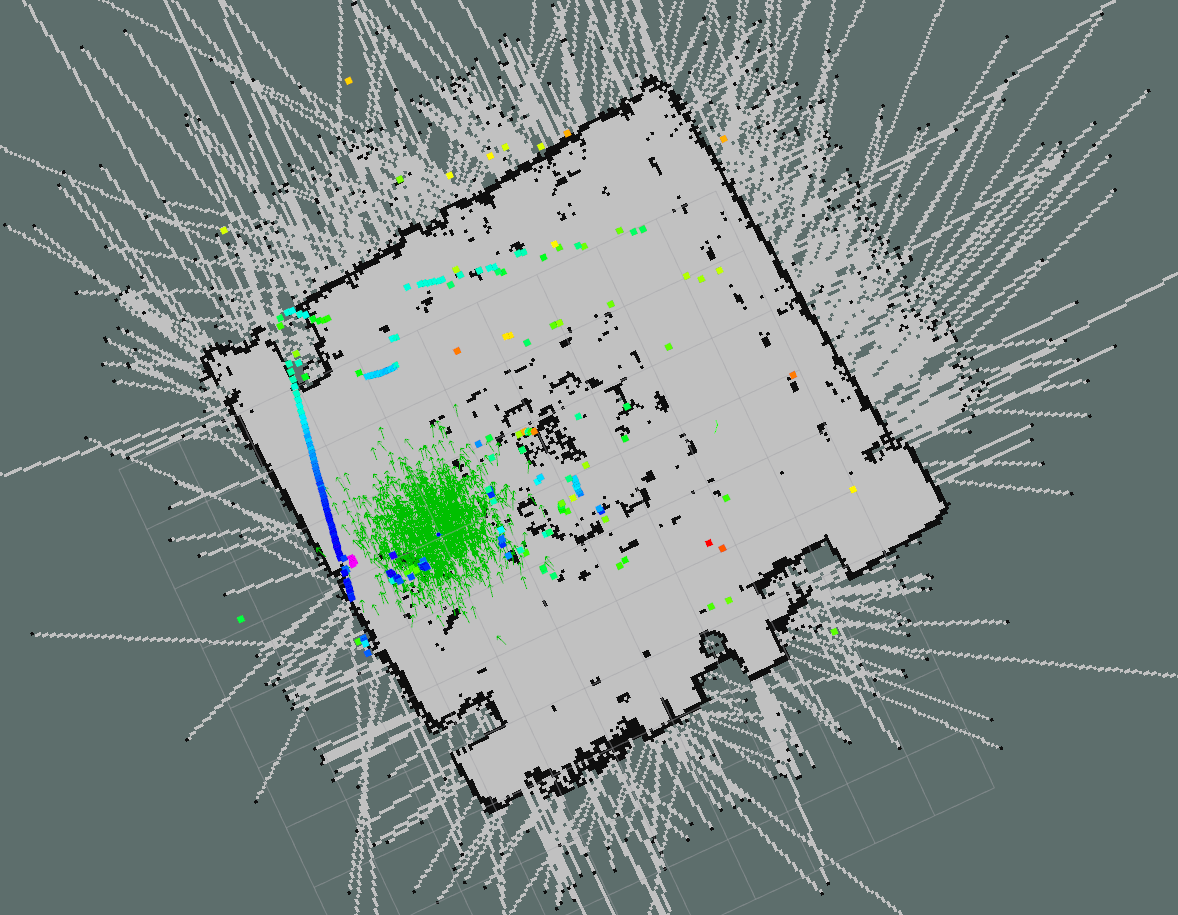
\includegraphics[width=0.7\linewidth, trim={4cm 5cm 12cm 6cm},clip]{img/Experiment3_Lokalisierung_1.png}
\caption{Ausgangszustand der Lokalisierung nach Positionsschätzung}
\end{figure}

Im nächsten Schritt der Navigation ein Zielpunkt in kurzer Distanz unmittelbar vor dem Roboter vorgegeben, woraufhin dieser die Bewegung startet. Während der Bewegung wird deutlich, dass sich der Mittelwert der Positionsschätzung verändert, was sich durch die Ausrichtung der Distanzmessungen zu dem Verlauf der Wände manifestiert. Dies zeigt sich in der nächsten Abbildung, wobei das Zusammenrücken der Partikel verdeutlicht, dass die Sicherheit der Lokalisierung zunimmt.
\begin{figure}[!ht]
\centering
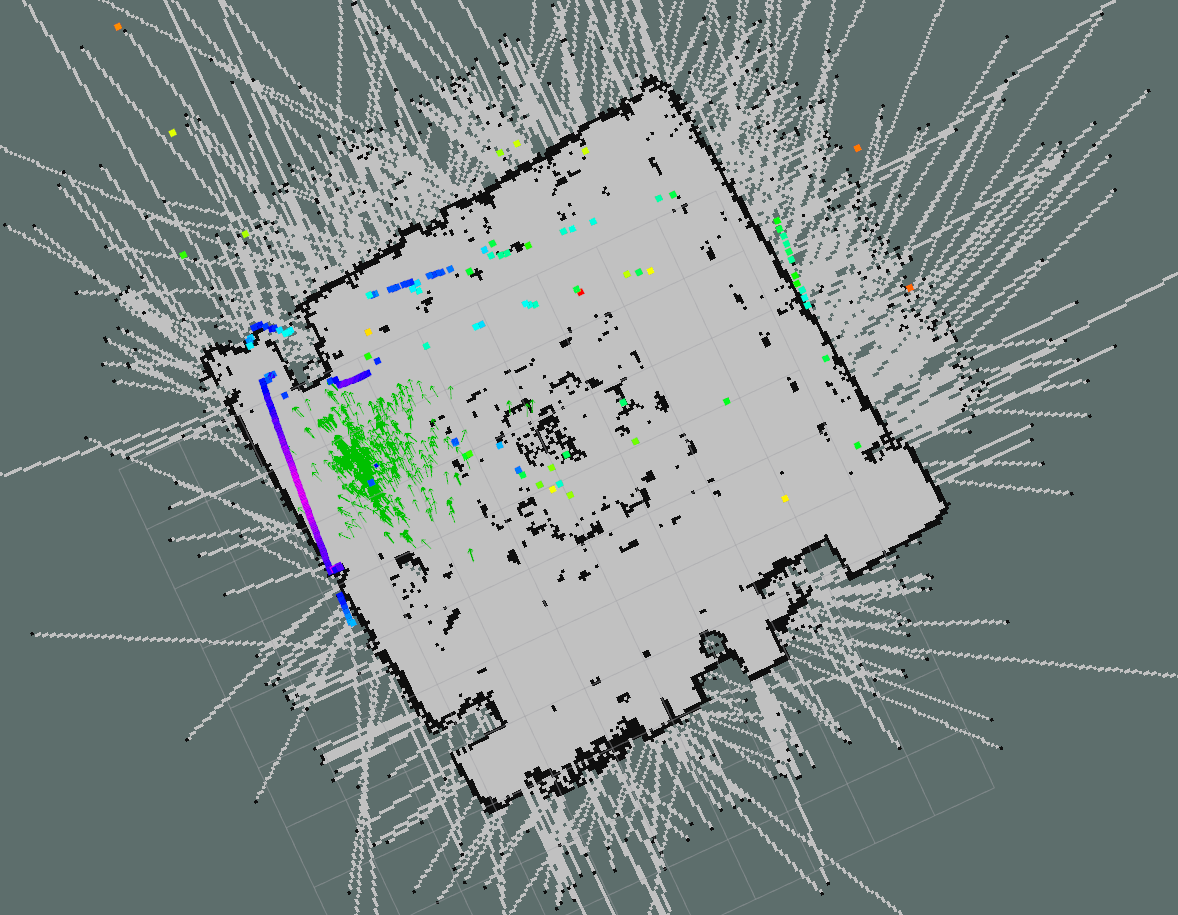
\includegraphics[width=0.7\linewidth, trim={4cm 5cm 12cm 6cm}, clip]{img/Experiment3_Lokalisierung_3.png}
\caption{Positionsschätzung nach kurzer Fahrdistanz}
\end{figure}

Die nächste Abbildung zeigt den Zustand der Lokalisierung in dem Moment, als der Zielpunkt erreicht wird. Nun stimmen die Punkte der Distanzmessung nahezu vollkommen mit den in der Karte eingezeichneten Hindernissen überein. Außerdem haben sich die Partikel weiter zusammengezogen, was für eine hohes Maß an Sicherheit der Lokalisierung spricht.
\begin{figure}[!ht]
\centering
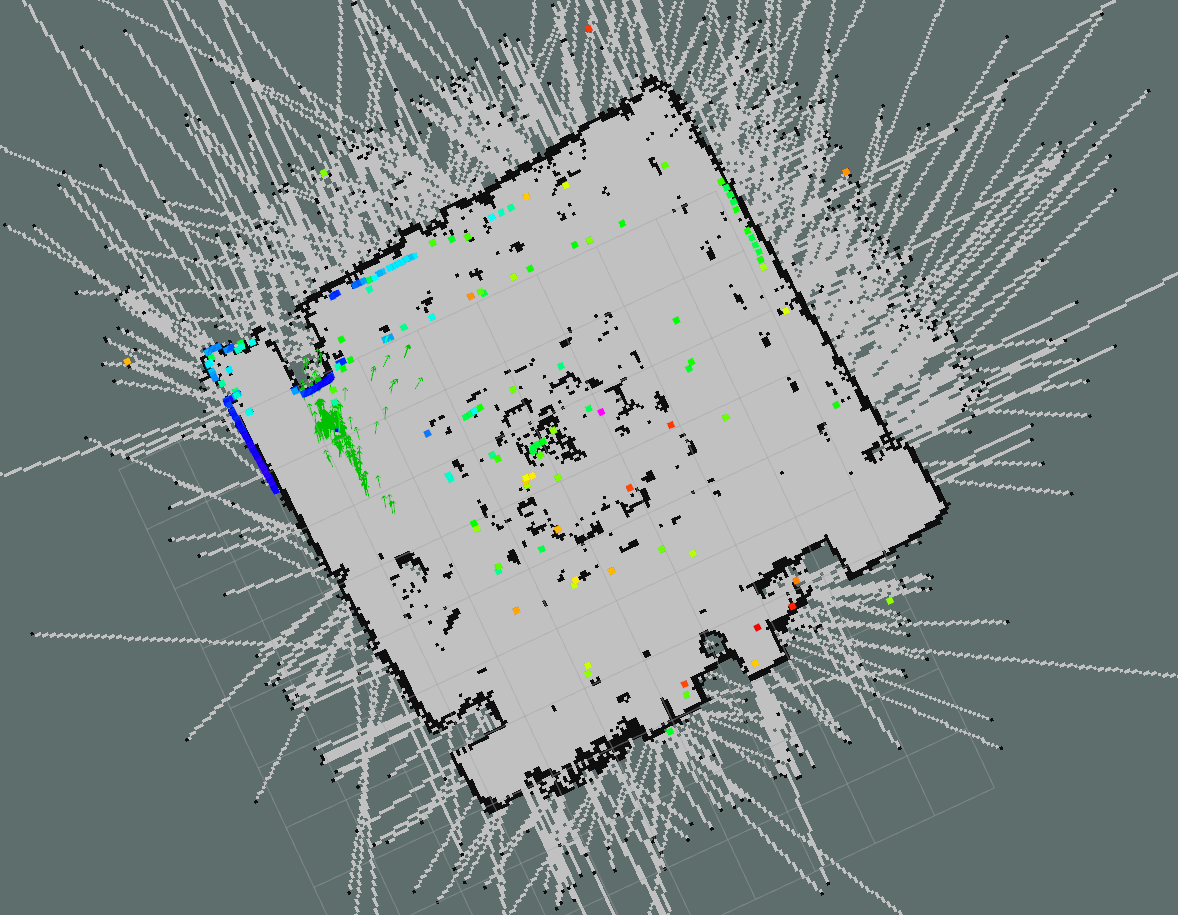
\includegraphics[width=0.7\linewidth, trim={4cm 5cm 12cm 6cm}, clip]{img/Experiment3_Lokalisierung_4.png}
\caption{Positionsschätzung bei Erreichen der Zielposition}
\end{figure}

Im letzten Schritt wird ein weiteres Navigationsziel gesetzt, woraufhin der Roboter sich weiter durch den Raum bewegt. Hier zeigt sich eine weitere Verdichtung der Partikelwolke, was sich darauf zurückführen lässt, dass die Distanzmessungen weiterhin mit der Karte übereinstimmen. Somit kann die Lokalisierung mit einem erhöhten Maß an Sicherheit als richtig angenommen werden.

An dieser Stelle sei eine negative Kopplung der Navigation und Lokalisierung erwähnt. Im Fall, dass die Lokalisierung in Form einer Positionsschätzung reinitialisiert wird und nur eine kurz entferntes Ziel angesteuert wird, wird während der Navigation die Position des Roboters durch den Lokalisierungsalgorithmus angepasst. Dies hat wiederum zur Folge, dass der Plan des Roboters überarbeitet werden muss, da die ursprüngliche Position verworfen wurde. Dies hat zur Folge, dass der Roboter wiederholte Rotationsmanöver ausführt, die von kurzen Translationsbewegung gefolgt werden. In diesem Muster bewegt sich der Roboter mehrere Male auf der Stelle, bis die Lokalisierung ein ausreichend hohes Maß an Sicherheit erreicht hat, sodass die geschätzte Position sich nur noch in einer für die Navigation nicht relevanten Größenordnung ändert.